\documentclass{standalone}
\usepackage{tikz}
\begin{document}
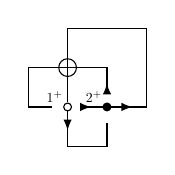
\begin{tikzpicture}[scale=.5]
  \node[circle, draw=black, inner sep=1pt] (1) at (0,0) {};
  \node[circle, draw=black, fill=black, inner sep=1pt] (2) at (1,0) {};
  \draw[] (-1,0) -- (-.4, 0) ;
  \draw[-latex] (.5, 0) -- (.6, 0);
  \draw[-latex] (.4,0) -- (2) -- (1.65,0);
  \draw[] (1.4, 0) -- (2,0) -- (2,2) -- (0, 2) -- (1);
  \draw[-latex] (1) -- (0, -.6);
  \draw[] (0,-.5) -- (0, -1) -- (1, -1) -- (1, -1) -- (1, -.4);
  \draw[-latex] (1, .4) -- (1,.6);
  \draw[] (1,.4) -- (1, 1) -- (-1, 1) -- (-1,0);

  \node[above left, scale=.5] () at (1) {$1^+$};
  \node[above left, scale=.5] () at (2) {$2^+$};
  \draw (0,1) circle (.225);
\end{tikzpicture}
\end{document}

% \documentclass{standalone}
% \usepackage{tikz}
% \begin{document}
% \begin{tikzpicture}[scale=.5]
%   \node[circle, draw=black, inner sep=1pt] (1) at (0,0) {};
%   \node[circle, draw=black, fill=black, inner sep=1pt] (2) at (2,0) {};
%   \draw[] (-1,0) -- (-.4, 0) ;
%   \draw[-latex] (.5, 0) -- (.6, 0);
%   \draw[-latex] (.4,0) -- (2) -- (2.65,0);
%   \draw[] (2.4, 0) -- (3,0) -- (3,2) -- (0, 2) -- (1);
%   \draw[-latex] (1) -- (0, -.6);
%   \draw[] (0,-.5) -- (0, -1) -- (1, -1) -- (1, 1) -- (2, 1) --
%   (2, .4);
%   \draw[-latex]  (2,-.4) -- (2,-.6);
%   \draw (2, -.5) -- (2, -2) -- (-1, -2) -- (-1,0);

%   \draw (1,0) circle (.225);

%   \node[above left, scale=.5] () at (1) {$1^+$};
%   \node[above left, scale=.5] () at (2) {$2^-$};

% \end{tikzpicture}
% \end{document}
